\graphicspath{ {GUI/} }
\chapter{Introduction}
\section{Background}

This project was initiated by Dr H.A.\ Engelbrecht to develop a lab tool with which a person can test
a topology's performance under various network conditions without having to set up the network\\

\section{Literature Study}
\section{Aims and Objectives}

\begin{enumerate}
\item Simulate various custom topologies under  user-defined network conditions.
\begin{enumerate}
\item Using all virual components (Hosts, switches, etc) over the emulated network.
\item Using some real components over the emulated network.
\end{enumerate}
\item Create a easy-to-use Graphical User Interface, to allow customization of:
\begin{enumerate}
\item Topology
\item Network conditions
\end{enumerate}
\item Allow user to save custom topologies
\item Test all custom topologies under same conditions
\item Stream a video and/or DHCP server over the network and to see accurate results
\item Create an accurate network simulator capable of:
\begin{enumerate}
\item Setting up network with it's conditions
\item Streaming over the network
\item Alternative testing of network conditions
\end{enumerate}
\end{enumerate}\newpage
\section{Graphical User Interface}
To ensure that the user gets the most out of the Mininet Network Emulator tool, it is important 
to allow the user to specify the network Topology and set various network conditions, like \textit{bandwidth}, \textit{delay},
\textit{Packet loss} and \textit{jitter}. As seen in figure 1.4.1, the main window consists of three widget frames, namely the \textbf{\textit{Hosts Widget}},  \textbf{\textit{Switches Widget}} and the  \textbf{\textit{Links Widget}}. Each of these widgets allow the user to add hosts and switches and to customize the link parameters for each host to a switch. Figure1.4.2 shows the inner workings of the GUI.
\begin{figure}[H]
    \centering
    \textbf{Mininet Network Emulator GUI}\par\medskip
    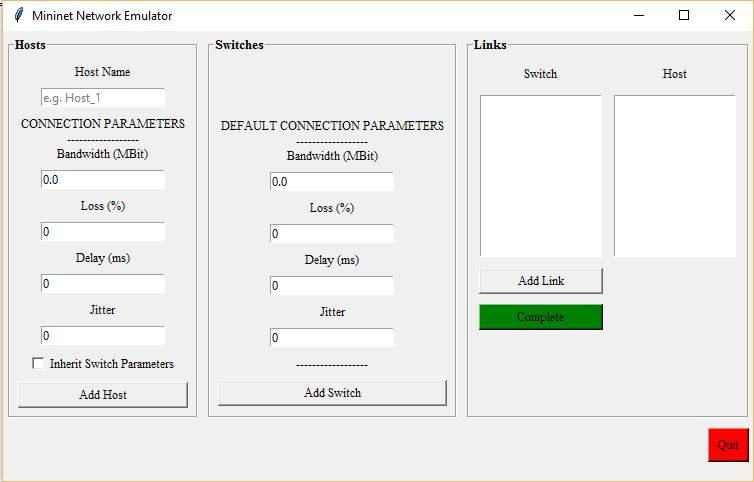
\includegraphics[scale=0.5]{Entire_window}
    \caption{Mininet Network Emulator GUI Frame}
\end{figure}
\begin{figure}[H]
    \centering
    \includegraphics[scale=0.5]{GUIflow}
    \caption{GUI flow chart}
\end{figure}

\subsection{Hosts Widget}
The Host widget essentialy allows the user to add host entities to the network. The user can customize the Host ID/Host Name by entering a name into the first
textfield. In the case that the user leaves the textfield blank, a default name \textit{'h1', 'h2', 'h3', etc} will be used. The user can also add connection parameters/non-idealities for each individual Host, \textit{bandwidth}, \textit{delay}, \textit{Packet loss} and \textit{jitter}, to simulate a real life connection. Value testing prevents the user from entering invalid parameters into textfields, like text and other ascii values, to ensure only valid entries are saved. Default values for all the connection parameters are 0. The radio button \textbf{\textit{Inherit Switch parameters}}, instantly changes the Host link parameters to inherit the switch's connection parameters when it is selected. When the \textbf{\textit{Add Host Button} }is pressed, the host name and all it's connection parameters are written into a text file \textit{'hosts.txt'}, which is then later used to create mininet objects- this will be discussed later in this document.\\
\begin{figure}[H]
\centering
\begin{minipage}{.5\textwidth}
  \centering
  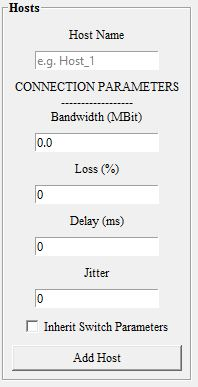
\includegraphics[width=.4\linewidth]{Hosts}
  \caption{Hosts widget}
  \label{fig:test1}
\end{minipage}%
\begin{minipage}{.5\textwidth}
  \centering
  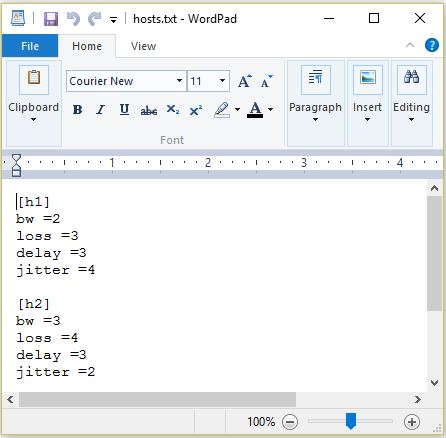
\includegraphics[width=.8\linewidth]{hosts_txt}
  \caption{Example of created Hosts text file}
  \label{fig:test2}
\end{minipage}
\end{figure}

\subsection{Switches Widget}
The Switches widget essentialy allows the user to add switch entities to the network. A default name \textit{'S1', 'S2', S3', etc} is automatically assigned to each switch entity. The user can also add connection parameters/non-idealities for each individual switch, \textit{bandwidth}, \textit{delay}, \textit{Packet loss} and \textit{jitter}, which is similar to the Host connection parameters but are only used when the user decides to add baseline parameters, which a link will inherit in the case that the Host connecting to the switch's parameters are 0. Value testing prevents the user from entering invalid parameters into textfields, like text and other ascii values, to ensure only valid entries are saved. Default values for all the connection parameters are 0. When the \textbf{\textit{Add Switch Button}} is pressed, the switch name an all it's connection parameters are written into a text file \textit{'switches.txt'}, which is then later used to create mininet objects- this will be discussed later in this document.\\
\begin{figure}[H]
\centering
\begin{minipage}{.5\textwidth}
  \centering
  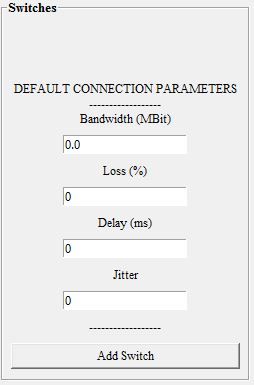
\includegraphics[width=.4\linewidth]{Switches}
  \caption{Hosts widget}
  \label{fig:test1}
\end{minipage}%
\begin{minipage}{.5\textwidth}
  \centering
  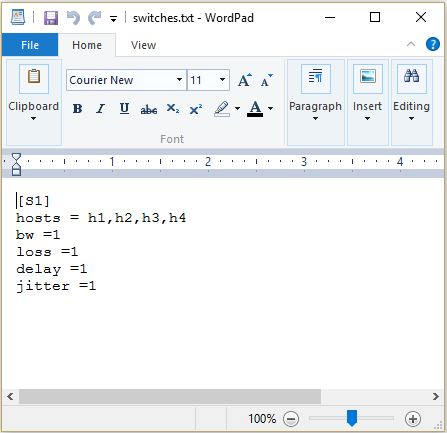
\includegraphics[width=.8\linewidth]{switches_txt}
  \caption{Example of created Switches text file}
  \label{fig:test2}
\end{minipage}
\end{figure}

\subsection{Links Widget}
The Links widget essentialy allows the user to link network entities, namey $x$ amount of hosts to 1 switch. As shown in figure 3, two Listboxes are used, the Host-listbox and the Switches-listbox, the user selects one or more hosts from the first listbox and then selects the switch they want to connect the hosts to. After they have decided which links they want make, the user can then click the \textbf{\textit{Add Link Button}} which will then save the Hosts connected to a specific switch and save it to the textfile \textit{'switches.txt'}, to indicate which entities are connected to one another.
\begin{figure}[H]
    \centering
    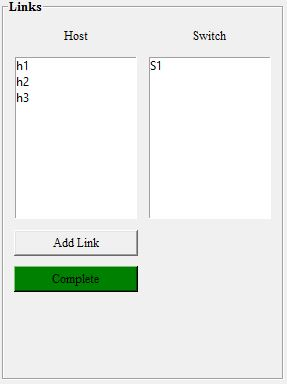
\includegraphics[scale=0.8]{Links}
    \caption{Links widget}
\end{figure}